\section*{Calendar-holdout velocity tests: preceding assessment}
No velocity profile is validated. Three parameterizations, each with six sensitivity runs, were fitted to the project's own pre-2025 arrivals. The 62-event, 1,065-arrival 2025 holdout is byte-for-byte unchanged. A three-layer trial with station delays fixed at zero improves conditional holdout prediction, but fails location and model stability tests. No new profile replaces the model behind Figure S6 or the earlier relocated catalog.

\subsection*{Diagnosis and observed-arrival review}
For the previous balanced fit, 186 held-out arrivals in 15 station/phase pairs absent from training account for 74.7\% of the added squared residual. Represented pairs account for 25.3\% and also deteriorate. Using all 490 eligible training events improves represented-pair RMS from 0.2349 to 0.2269 s, but worsens unrepresented-pair RMS from 0.2685 to 0.4397 s. Missing station support is therefore consequential but does not explain every failure.

The old fitted velocities with zero station delays give holdout RMS 0.2642 s. The old delays with initial velocities give 0.3604 s, compared with 0.2778 s for the coupled old fit and 0.2406 s for its initialization. These are conditional counterfactual tests with relocated holdout sources; they demonstrate a velocity--delay tradeoff, not a unique causal decomposition.

Visual inspection covered 24 original three-component arrival windows (12 training, 12 holdout), with one valid response epoch for each of 72 channel windows. Six onsets were visually consistent; 18 were ambiguous. These are AI judgments, not human seismologist review or verified phase identities. No pick was shifted or deleted. Four network gathers further inspect unstable events 225, 1532, 2403 and 2642. Training event 1532 has many assigned P arrivals within a pre-existing decaying packet; a separate leave-one-event-out sensitivity tests its influence without declaring it false. Both held-out network examples retain coherent packets with some ambiguous phases and remain in the holdout.

\subsection*{Parameterization and unchanged tests}
The primary training subset contains 52 events and 827 arrivals (366 P, 461 S); a selection sensitivity contains 62 events and 990 arrivals. Training spans 11 sampled days from 21 January 2022 to 20 May 2024. Selection stratifies each day by 1-km provisional depth bins, then supplements rare training station/phase combinations. It covers all 35 training combinations found in the holdout; 11 holdout combinations, totaling 172 arrivals, remain unsupported. No qualifying late-2024 calibration event exists in this frozen checkpoint. Unrelated background downloads and picks do not enter the fit.

Four layers retain tops at $-0.5,0.5,1,3$ km below sea level. Two three-layer alternatives merge the shallow layers, with tops at $-0.5,1,3$ km and initial $V_p=(1.8,3.0,5.5)$ km/s. All initialize $V_p/V_s=1.78$ from the disclosed Tramelli et al. (2021) alternative; both velocities subsequently float. The bottom layer is a halfspace. Two families fit station delays with damping 10, compared with 0.1 previously; the third fixes delays at zero, a deliberate restrictive departure from Tan's joint inversion. No low-velocity layers are allowed. P/S weights are 1/0.5; layer damping is 10; origin, horizontal, depth and velocity damping are 0.01, 0.1, 0.1 and 1. Maximum depth/velocity updates remain 0.2 km and 0.1 km/s.

Each fit has 21 fixed prelocation iterations, 14 velocity-only iterations and five joint 14-iteration blocks. The last two blocks test additional iterations. Sensitivities change starting velocities by $\pm5\%$, training selection, velocity damping by a factor of 10, and arithmetic precision. Holdout locations and origin times are fitted for 35 iterations with velocities and delays fixed, followed by 35 more as a convergence check. This is conditional arrival prediction, not an independent measurement of absolute location. Previously inspected holdout diagnostics informed the study design, so this is a reused validation set rather than a pristine final test. All registered results are reported.

Acceptance still requires improved holdout RMS, physically admissible velocities and stability within 100 m horizontally, 0.1 km in depth, 0.05 km/s in velocity and 0.02 s in delays. No threshold was relaxed. Additional convergence checks supplement those requirements.

\begin{center}\small
\begin{tabular}{lcc}\toprule
Model & Training RMS, initial / fitted (s) & Holdout RMS, initial / fitted (s)\\\midrule
Four layers, damped delays & 0.2166 / 0.1778 & 0.2406 / 0.2416\\
Three layers, damped delays & 0.2169 / 0.1801 & 0.2432 / 0.2413\\
Three layers, zero delays & 0.2169 / 0.2118 & 0.2432 / 0.2274\\
\bottomrule\end{tabular}\end{center}

\begin{center}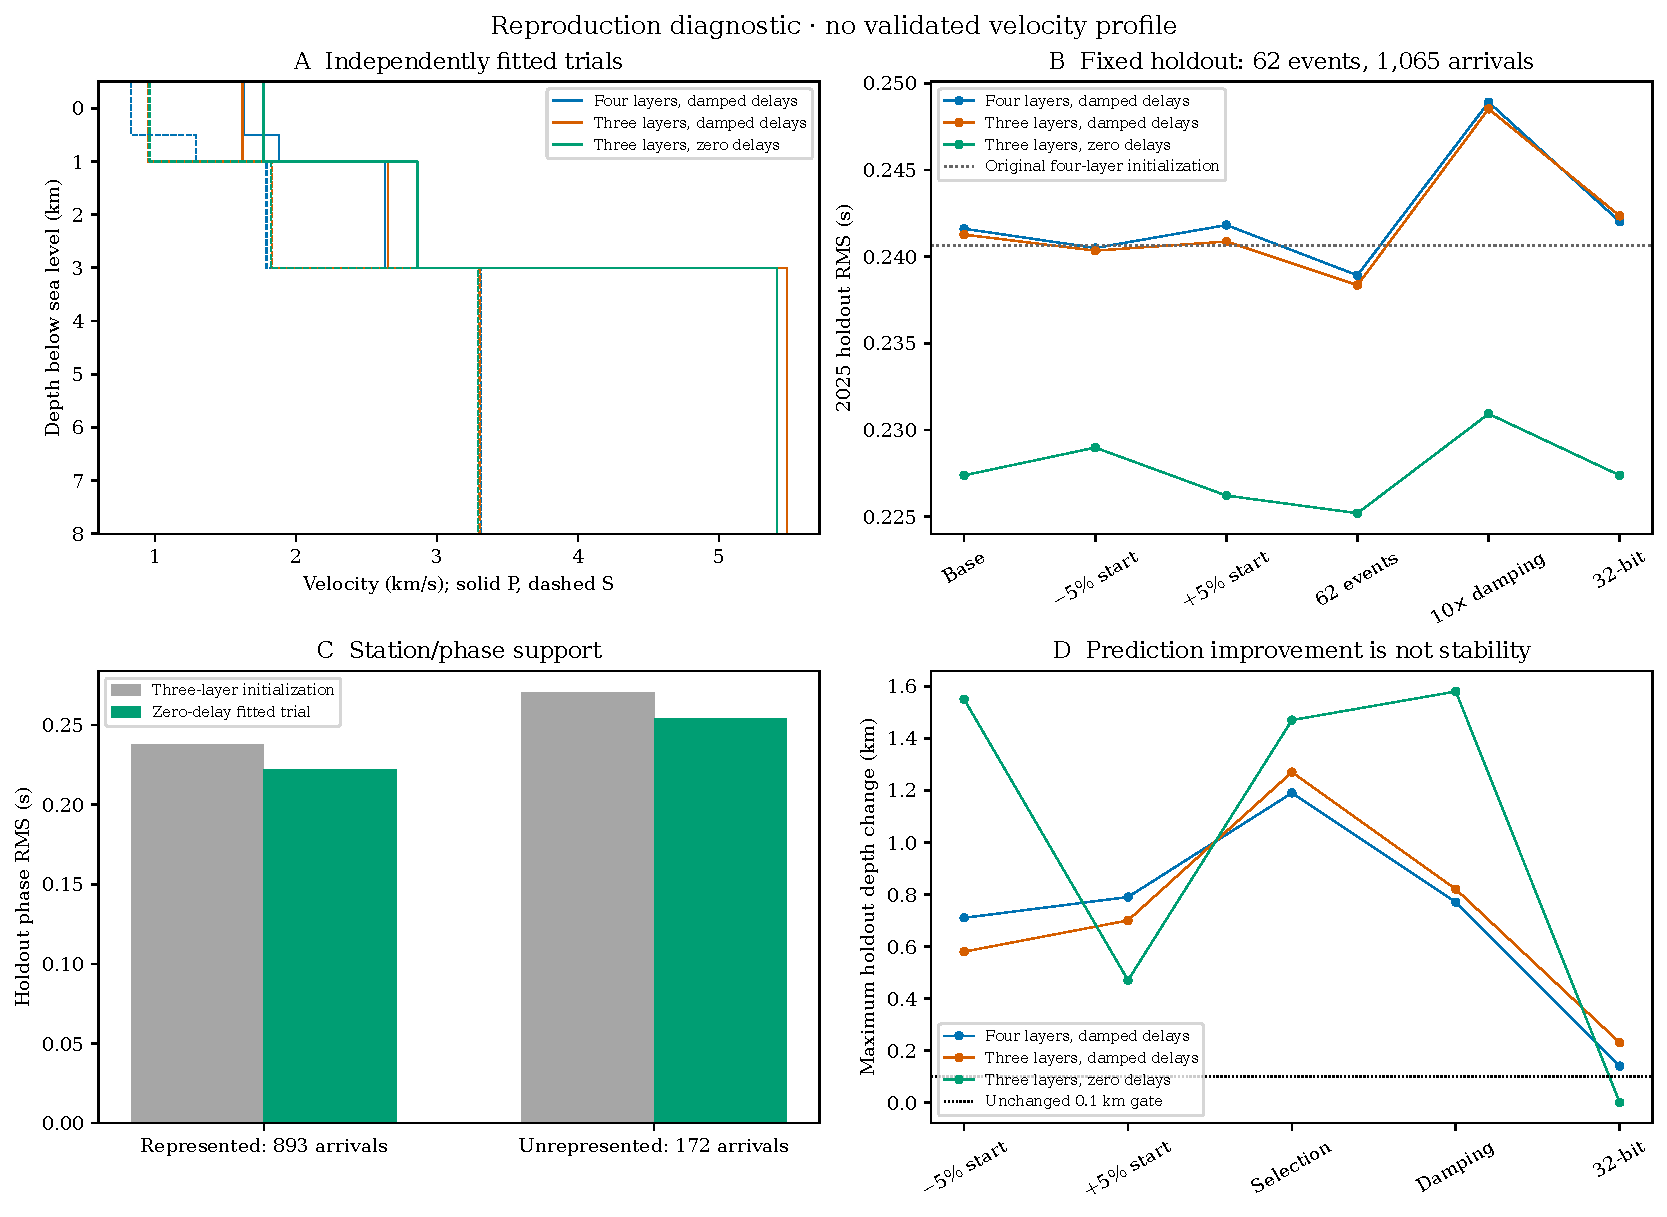
\includegraphics[width=\linewidth]{figures/velocity_holdout_diagnostic.pdf}\end{center}
Reproduction diagnostic, not a paper panel. Every curve comes from saved independent model or residual outputs. Sensitivity changes are not confidence intervals.

\subsection*{Improved prediction with unresolved locations}
The zero-delay base trial improves holdout RMS from 0.2432 to 0.2274 s, also below the original four-layer baseline of 0.2406 s. Represented-pair RMS decreases from 0.2376 to 0.2219 s; unrepresented-pair RMS decreases from 0.2705 to 0.2541 s. Four of five sampled holdout days improve; 1 February worsens from 0.1208 to 0.1258 s. Across six zero-delay sensitivities, holdout RMS ranges from 0.2252 to 0.2309 s. Thus prediction improves without establishing a unique velocity profile.

The zero-delay base profile has $(V_p,V_s)=(1.77,0.96),(2.86,1.82),(5.41,3.29)$ km/s in the three layers. It is monotonic with positive isotropic bulk modulus; these necessary physical checks do not establish correctness. Its 32-/64-bit printed profiles and held-out locations agree, but initialization, selection and damping still change held-out depths by up to 1.58 km, horizontal positions by 800 m and velocities by 0.28 km/s. Between the third and fifth joint blocks, training locations change by 409 m and 0.18 km. The extra holdout pass moves four events more than 100 m horizontally and seven more than 0.1 km vertically. Event 2403 moves from 3.00 to 2.18 km and by 780 m horizontally; event 2642 crosses the 3-km interface in the other direction. These exceed the unchanged gates even though total RMS changes little.

The training-only sensitivity omitting ambiguous event 1532 uses 51 events. Its holdout RMS is 0.2287 s; an additional holdout pass still changes depth by 0.57 km and horizontal position by 245 m. It does not resolve the validation failure.


\begin{center}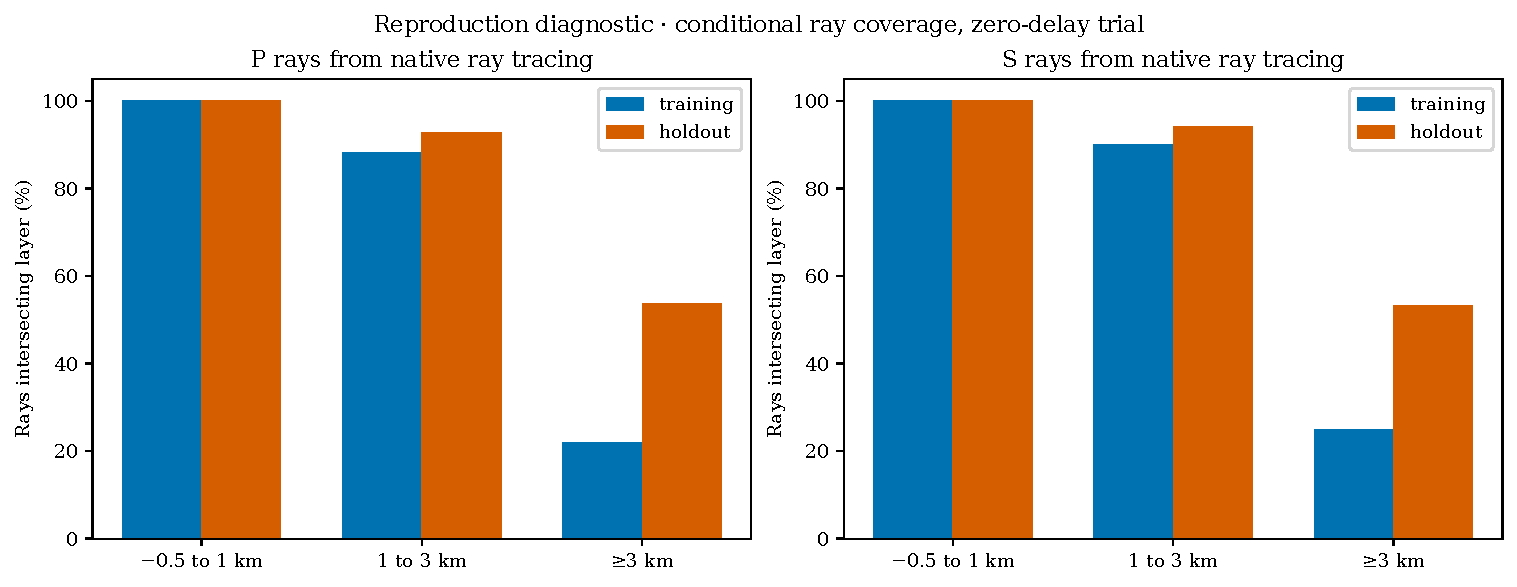
\includegraphics[width=.92\linewidth]{figures/velocity_ray_coverage.pdf}\end{center}
Reproduction diagnostic. In the zero-delay trial, only 80/366 training P rays and 115/461 training S rays enter the layer at or below 3 km, compared with 223/415 and 347/650 in the holdout. Ten training source estimates and 23 held-out source estimates lie in that layer. These conditional geometries demonstrate a substantial depth-coverage mismatch; they are not independently known event depths. Native ray vertices match output source depths to their 0.01-km precision. Independently summed path travel times differ from saved residual predictions by RMS 0.0038--0.0075 s, including rounded vertices, velocities, origin times and delays. The generic aggregate two-model ray table has inconsistent layer counts (86 sources for a 46-event prior run); it is not used. Per-ray files are matched to every phase token instead.

\subsection*{Specific work still needed}
Review the ambiguous training onsets and associations, beginning with event 1532 and the saved 24 windows. A reviewed reference must be independent of model residual minimization. If holdout labels later change after expert review, preserve this frozen test and report both versions; do not retrospectively remove failures. Additional pre-2025 coincident arrivals should support 2I.CGAU P, S; 2I.CLAC S; 2I.CREM P, S; 2I.CSOC P, S; IV.CRUS P, S; IV.CUMA P, S. The four 2I stations require eligible events in late-2024 HH-channel intervals advertised by EIDA, with common IV stations. StationXML contains earlier station epochs for CGAU and CSOC; station epochs alone do not establish waveform availability. Better resolved source depths and rays spanning the 3-km interface are also needed. A sufficient event count cannot be inferred from these trials. Sparse days and ambiguous phases limit generalization even when aggregate residuals improve.

\subsection*{Evidence and rebuild}
\begingroup\footnotesize
\path{data/velocity_holdout_review/experiment_plan.json}\par
\path{data/velocity_holdout_review/experiment_results.csv}\par
\path{data/velocity_holdout_review/station_phase_residuals.csv}\par
\path{data/velocity_holdout_review/iteration_event_stability.csv}\par
\path{data/velocity_holdout_review/ray_coverage.csv}\par
\path{data/velocity_holdout_review/review/decisions.csv}\par
\path{data/velocity_holdout_review/review/network_decisions.json}\par
\path{docs/VELOCITY_HOLDOUT_REVIEW.md}\par
\path{scripts/rebuild_velocity_holdout.py}\par
\endgroup
All numerical trials and failed gates remain saved. Figures 2--4 and S6 retain their explicitly identified earlier numerical checkpoints; no location, relocation, magnitude or mechanism has been promoted using an unvalidated profile. Published reference images remain confined to the separate comparison PDF. The earlier assessment below is preserved as the history of the failed four-layer model.
